\let\negmedspace\undefined
\let\negthickspace\undefined
\documentclass[journal]{IEEEtran}
\usepackage[a5paper, margin=10mm, onecolumn]{geometry}
\usepackage{lmodern} % Ensure lmodern is loaded for pdflatex
\usepackage{tfrupee} % Include tfrupee package

\setlength{\headheight}{1cm} % Set the height of the header box
\setlength{\headsep}{0mm}     % Set the distance between the header box and the top of the text

\usepackage{gvv-book}
\usepackage{gvv}
\usepackage{cite}
\usepackage{amsmath,amssymb,amsfonts,amsthm}
\usepackage{algorithmic}
\usepackage{graphicx}
\usepackage{textcomp}
\usepackage{xcolor}
\usepackage{txfonts}
\usepackage{listings}
\usepackage{enumitem}
\usepackage{mathtools}
\usepackage{gensymb}
\usepackage{comment}
\usepackage[breaklinks=true]{hyperref}
\usepackage{tkz-euclide} 
\usepackage{listings}
\usepackage{gvv}                                        
\def\inputGnumericTable{}                                 
\usepackage[latin1]{inputenc}                                
\usepackage{color}                                            
\usepackage{array}                                            
\usepackage{longtable}                                       
\usepackage{calc}                                             
\usepackage{multirow}                                         
\usepackage{hhline}                                           
\usepackage{ifthen}                                           
\usepackage{lscape}
\begin{document}

\bibliographystyle{IEEEtran}
\vspace{3cm}

\title{4.4.2.14}
\author{EE24BTECH11010 - Balaji B}
% \maketitle
% \newpage
% \bigskip
{\let\newpage\relax\maketitle}
\textbf{Question:}\\
Show that two lines $a_1x+b_1y+c_1 = 0 \text{ and } a_2+b_2+c_2=0 \text{ where } b_1b_2 \neq 0$ are Perpendicular if $a_1a_2 + b_1b_2 = 0.$\\
\textbf{Answer:}\\
\begin{table}[h!]    
  \centering
  \begin{tabular}[12pt]{ |c| c| c|c|c|c|}
    \hline
    $X$ & 1 & 2 & 3 & 4 & 5 \\
    \hline
    $P(X)$ & $K$ & 2$K$ & 2$K$ & 3$K$ & $K$ \\
    \hline 
    \end{tabular} 

  \caption{Variables Used}
  \label{tab1-1.9-6}
  \end{table}\\
The equation of line is given by,
\begin{align}
    y &= mx + c \\
    x &= x\\
    \myvec{x \\ y} &= x\myvec{1 \\ m} + \myvec{0\\c}\\
    \vec{x} &= k\vec{m} + \vec{h}
\end{align}
Writing the line \textbf{1} in the form of the above equation, we get
\begin{align}
    a_1x+b_1y+c_1 = 0\\
    y = -\frac{a_1}{b_1} x -\frac{c_1}{b_1}\\
    \vec{x} = x\myvec{1 \\ -\frac{a_1}{b_1}} + \myvec{0 \\ -\frac{c_1}{b_1}}\\
\therefore \vec{m_1} = \myvec{1\\-\frac{a_1}{b_1}}
\end{align}
Writing the line \textbf{2} in the form of the above equation, we get
\begin{align}
    a_2x+b_2y+c_2 = 0\\
    y = -\frac{a_2}{b_2} x -\frac{c_2}{b_2}\\
    \vec{x} = x\myvec{1 \\ -\frac{a_2}{b_2}} + \myvec{0 \\ -\frac{c_2}{b_2}}\\
\therefore \vec{m_2} = \myvec{1\\-\frac{a_2}{b_2}}
\end{align}
For the lines to be perpendicular $m_1^\top m_2 = 0.$\label{eq1.5.37.1}
\begin{align}
    \myvec{1 && -\frac{a_1}{b_1}}\myvec{1 \\ -\frac{a_2}{b_2}} = 0\\
    1 + \frac{a_1}{b_1}\frac{a_2}{b_2} = 0\\
    a_1a_2 + b_1b_2 = 0
\end{align}
Let's consider $a_1 = 1, b_1 = 1, c_1 = 0$ and 
$a_2 = 1, b_2 = -1, c_2 =0. $\\ \\
The equation of line \textbf{1} will be
\begin{align}
\vec{x} = x\myvec{1 \\ -1} + \myvec{0 \\ 0}
\end{align}
The equation of line \textbf{2} will be
\begin{align}
\vec{x} = x\myvec{1 \\ 1} + \myvec{0 \\ 0}
\end{align}
From above we have $m_1 = \myvec{1 \\-1 } \text{ and } m_2 = \myvec{1 \\ 1} $ \\
For lines to be perpendicular:
\begin{align}
    \myvec{1 && -1}\myvec{1\\ 1} = 0    
\end{align}
 $\therefore$ The lines are perpendicular.

 \begin{figure}[h!]
   \centering
   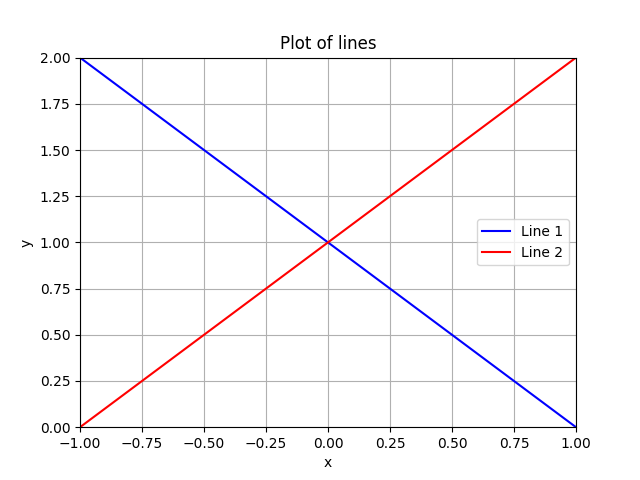
\includegraphics[width=0.7\linewidth]{figs/fig.png}
   \caption{Plot of two perpendicular lines}
   \label{stemplot}
\end{figure}
\end{document}



